\documentclass[main.tex]{subfiles}
\begin{document}

\marginpar{Wednesday\\ 2020-11-4, \\ compiled \\ \today}

We were discussing the flow of plasma from the donor star to the compact object through the inner Lagrangian point.
The velocities of the compact object in the frame of the gas are \(v_\parallel \sim \SI{10}{km/s}\) and \(v_\perp \sim \SI{100}{km/s}\), so we neglect \(v_{\parallel}\).

Suppose we have a mass \(M\), and a particle in a bound orbit around this mass.
Its energy \(E\) and energy per unit mass \(\epsilon \) will be 
%
\begin{align}
E = - \frac{GMm}{2a} && \epsilon = - \frac{GM}{2a} 
\,,
\end{align}
%
while its specific angular momentum will be (in terms of the eccentricity \(e\)):
%
\begin{align}
\qty( \frac{L}{m})^2 = \ell^2 = (1 - e^2) GMa
\,.
\end{align}

Then, we can write the semimajor axis as 
%
\begin{align}
\frac{1}{a} = \frac{(1-e^2) GM}{\ell^2}
\,,
\end{align}
%
so the specific energy will read
%mk
\begin{align}
\epsilon = - \frac{GM (1-e^2) GM}{2\ell^2}= - \frac{(GM)^2(1-e^2)}{2 \ell^2}
\,.
\end{align}

We can ask ourselves: what is the orbit which has the minimum energy \(\epsilon _{\text{min}}\) at fixed \(\ell\)? The only thing which can vary is the eccentricity \(e\), so the minimum energy is attained for the circular orbit, with \(e = 0\), where 
%
\begin{align}
\epsilon _{\text{min}} = -\frac{(GM)^2}{2 \ell^2}
\,.
\end{align}

The stream of gas will be subjected to frictional forces, which will dissipate energy, and since the energy of circular orbits is minimum this will circularize the orbit. 
We will discuss the timescale of this process later.

We can estimate the radius of circularization, \(R _{\text{circ}}\): we know that for a circular orbit the angular momentum will reach its Keplerian value, \(L_k\), and the velocity will reach its Keplerian value. 
This reads 
%
\begin{align}
v_K = \sqrt{ \frac{GM}{R}} 
\,,
\end{align}
%
which comes from equating \(v^2 /R\) and \(GM/ R^2\).
The Keplerian (specific!) angular momentum reads 
%
\begin{align}
L_K = R v_K 
\,,
\end{align}
%
which we can compute at \(R _{\text{circ}}\): 
%
\begin{align}
L_K (R _{\text{circ}}) = \sqrt{GM R _{\text{circ}}}
\,.
\end{align}

If we fix the specific angular momentum \(\ell\) of an incoming fluid parcel we can then determine the radius of its orbit, \(R _{\text{circ}} = \ell^2 / GM\). 

We can compute this initial value of \(\ell\) since the velocity of the fluid is given by the \(v_{\perp} = \omega b_1 \), and then \(\ell = v_\perp b_1 = \omega b_1^2\). 
Then, finally, we have 
%
\begin{align}
R _{\text{circ}} = \frac{\omega^2 b_1^{4}}{GM} = \frac{4 \pi^2 b_1^{4}}{GM P^2}
\,.
\end{align}

In units of the orbital separation, and using Kepler's law 
%
\begin{align}
\omega^2 = \frac{G (M_1 + M_2 )}{a^3}
\,
\end{align}
%
we get (now denoting, more specifically, as \(M_1 \) the mass we previously just called \(M\)):
%
\begin{align}
\frac{R _{\text{circ}}}{a} &= \frac{\omega^2 b_1^{4}}{GM_1  a}  \\
&= \frac{b_1^{4} G (M_1 + M_2 )}{GM_1 a^{4}} = \qty(\frac{b_1 }{a})^{4} (1 + q)
\,.
\end{align}

Yesterday we saw that \cite[]{frankAccretionPowerAstrophysics2002}:
%
\begin{align}
\frac{b_1 }{a} \approx \num{.5} - \num{.227} \log q
\,,
\end{align}
%
using which we get 
%
\begin{align}
\frac{R _{\text{circ}}}{a} \approx \qty(\num{.5} - \num{.227} \log q)^{4} (1+q)
\,,
\end{align}
%
and we can also calculate the radius of the Roche lobe by inverting a result from yesterday (with \(q \to 1/q\)): 
%
\begin{align}
\frac{R_1}{a} = \begin{cases}
    \num{.38} -\num{.2} \log q & \num{.05} < q < 2 \\
    \frac{\num{.426}}{(1 + q)^{1/3}} & q > 2
\end{cases}
\,.
\end{align}

We can then see that \(R _{\text{circ}}\) is at least 10 times smaller than the radius of the lobe.

\begin{figure}[ht]
\centering
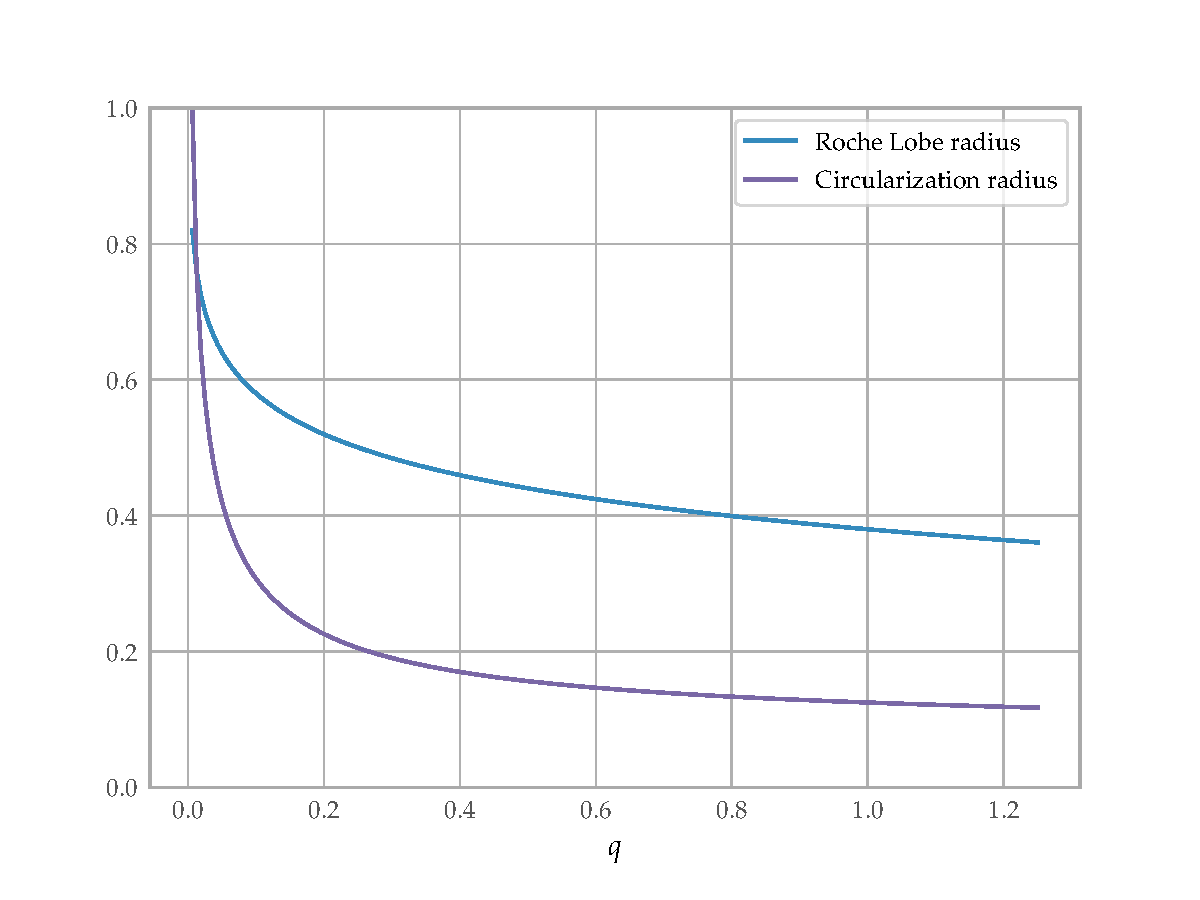
\includegraphics[width=\textwidth]{figures/roche-vs-circularization}
\caption{Roche lobe of star 1 versus circularization radius; both are plotted as \(R / a\).}
\label{fig:roche-vs-circularization}
\end{figure}

For a star we would need to ensure that \(R _{\text{circ}} > R_{*}\), but for a compact object there are no issues.

\subsection{The accretion disk}

Particles at their Keplerian velocities and radii around the compact object would keep orbiting, were it not for dissipative effects, which allow for energy and momentum to be transmitted throughout the disk.
% If we had two concentric disks, both of which 

There are three characteristic times we need to account for: 
%
\begin{align}
t _{\text{dyn}} < t _{\text{rad}} < t _{\text{visc}}
\,,
\end{align}
%
the dynamical, radiative and viscous timescale. Injection happens on a short \(t _{\text{dyn}}\) timescale, circularization happens on a longer \(t _{\text{rad}}\) timescale, shrinkage happens on an even longer \(t _{\text{visc}}\) timescale.

The true trajectory of a fluid element will be a spiral, which we can approximate with a succession of circles.
This is how an accretion disk forms. 

Since \(M _{\text{disc}} \ll M_1 \), the self-gravity of the accretion disk is negligible. Therefore, the azimuthal velocity of matter in the disk will closely match the Keplerian velocity 
%
\begin{align}
v_{\phi } = v_K = \sqrt{ \frac{GM_1}{R}}
\,.
\end{align}

We can already estimate the efficiency of the accretion process: the specific energy of the gas at the inner radius of the disk, \(R _{\text{in}}\), which is the star radius for a NS and the ISCO for a BH. 
The specific energy is 
%
\begin{align}
\epsilon (R _{\text{in}}) = - \frac{GM_1 }{R _{\text{in}}} 
+ \frac{1}{2} v_K^2 = - \frac{1}{2} \frac{GM_1 }{R _{\text{in}}}
\,.
\end{align}

The variation of the energy can be calculated starting from infinity since \(R_1 \gg R _{\text{in}}\):\footnote{This is a classical estimate, but it works well enough: for example, for a Schwarzschild BH we have calculated explicitly \(\epsilon _\infty - \epsilon (R _{\text{in}}) = 1 - \sqrt{8/9} \approx \SI{6}{\percent}\), while this expression would give \(1/12 \approx \SI{8}{\percent}\). Not strictly correct, but in the right ballpark.}
%
\begin{align}
\epsilon_{\infty } - \epsilon (R _{\text{in}}) = \frac{1}{2} \frac{GM_1}{R _{\text{in}}}
\,,
\end{align}
%
therefore the luminosity of the disk will be 
%
\begin{align}
L _{\text{disc}}= \frac{1}{2} \frac{GM_1 }{R _{\text{circ}}} \dot{M} c^2
\,,
\end{align}
%
only half of the accretion luminosity, defined as
%
\begin{align}
L _{\text{acc}} = \frac{GM_1 }{R _{\text{in}}} \dot{M} c^2
\,.
\end{align}

Now we want to make more detailed predictions.
A key point is viscosity: friction between the various gas elements.

Let us consider two layers of the disk.
They will have a macroscopic bulk motion, with \(v_\phi = R \Omega(R) \),
superimposed with a microscopic motion which can be at very small, up to mesoscopic scales. 
We can have micro-scale motion of ions, but also
medium-scale structures can form: turbulent eddies, since the Reynolds number can be shown to be very large.

\begin{figure}[ht]
\centering
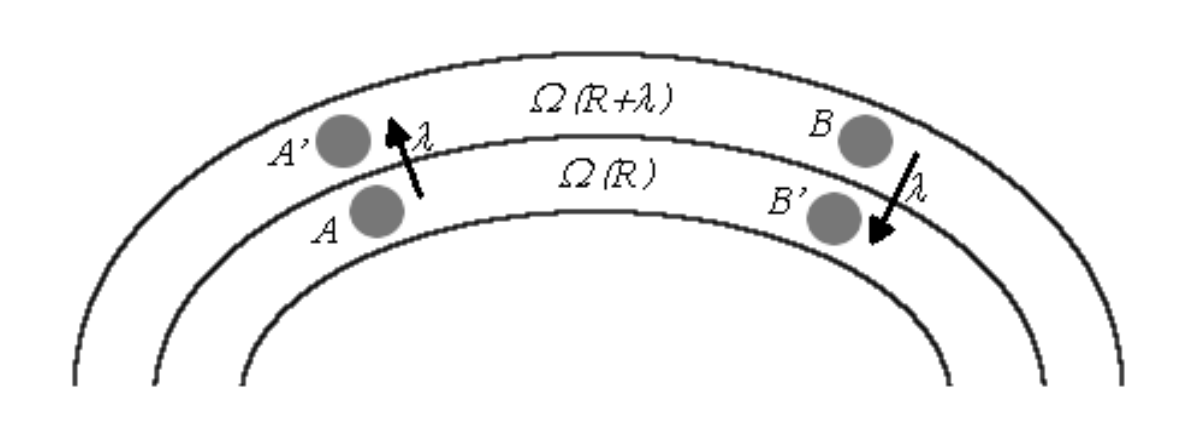
\includegraphics[width=\textwidth]{figures/turbulent-eddies-accretion}
\caption{Turbulent eddies moving.}
\label{fig:turbulent-eddies-accretion}
\end{figure}

Suppose we have an eddy which starts in \(A\), moves radially, and then dissipates in \(A'\).
Further, let us say that the length scale of its motion is \(\lambda \), and the typical velocity of its motion across the disk is \(\overline{v}\). 

Its radius and velocity at \(A\) will be \(R, \Omega(R) \times  R\); at \(A'\) they will be \(R + \lambda \) and still \(\Omega (R) \times R\). 

In terms of specific angular momentum, when the eddy dies it will dissipate angular momentum \((R+\lambda) R \Omega (R) \).

For an eddy moving from \(B\) to \(B'\) in the opposite direction we will have \(R (R + \lambda ) \Omega (R + \lambda )\). 
Since the motion is thermal, on average there will be as many particles going in both direction.

% \todo[inline]{But there is more volume at higher \(R\), so more matter!}

Suppose that the height of the disk is \(H\): then the mass per unit time carried by the eddies will be \(H 2 \pi R \overline{v} \rho \). 

Then, the variation of angular momentum will be 
%
\begin{align}
\frac{\Delta L}{\Delta t} &= 2 \pi R H \rho \overline{v} 
\qty[R (R + \lambda ) \Omega (R) - R (R+\lambda ) \Omega (R + \lambda )]  \\
&\approx - 2 \pi R^2 (R+ \lambda ) H \rho \overline{v} \dv{\Omega }{R} \lambda  \\
&\approx - 2\pi R^3 H \rho \overline{v} \lambda \dv{\Omega }{R}
\,,
\end{align}
%
and if we introduce the surface density of the disk: 
%
\begin{align}
\Sigma = \int_{- H/2 }^{H/2} \rho \dd{z} \approx \rho H
\,
\end{align}
%
we can write this torque as
%
\begin{align}
\frac{ \Delta L}{\Delta t} = \tau \approx -2 \pi R \Sigma \qty(\overline{v} \lambda ) R^2 \dv{\Omega }{R}
\,.
\end{align}

For a Keplerian accretion disk we always have \(\dv*{\Omega }{R} < 0\), since \(\Omega _K = \sqrt{GM / R^3}\): this means that the torque is positive.
Note, however, that we are still only considering the effect on a certain layer of the one above it --- this is not the full picture yet.

This is the torque which the inner part of the disk exerts on the outer part, decelerating it. 
We can then introduce a function \(G(R) = - \tau \), the torque exerted by the outer part of the disk on the inner part, accelerating it. 

For a given layer rotating at \(R \Omega (R)\), the layers above it will try to accelerate it, while the ones below it will try to decelerate it. What will be the net effect? It will be\footnote{We use the same letter \(\tau \) as before, but we should specify that this time it accounts for all the contributions to a certain layer of the disk, while before it was only one-way.}
%
\begin{align}
\tau =  G(R + \dd{R}) - G(R) = \dv{G}{R} \dd{R}
\,.
\end{align}

These opposite effects will dissipate heat. 
The differential work dissipated will be given by 
%
\begin{align}
\dd{W} = \tau \dd{\phi } = \dv{G}{R} \dd{R} \dd{\phi }
\,,
\end{align}
%
so, since to a first approximation \(G\) can be taken to be a constant, the power will be 
%
\begin{align}
\dv{W}{t} = \dv{G}{R} \dd{R} \Omega 
\,.
\end{align}

Integrating to find the total power we get
%
\begin{align}
\dot{E} &= \int_{R _{\text{in}}}^{R _{\text{out}} } \dv{G}{R} \Omega \dd{R} 
\,,
\end{align}
%
but we can integrate by parts to find 
%
\begin{align}
\dot{E} &= \eval{G \Omega }_{R _{\text{in}}}^{R _{\text{out}}}
- \int_{R _{\text{in}}}^{R _{\text{out}}} G \dv{\Omega }{R} \dd{R} 
\,,
\end{align}
%
so we can identify a global, \emph{convective term}: the variation of \(G \Omega \). On the other hand \(G \dv*{\Omega }{R} \dd{R}\) is a local dissipation term. 

Let us introduce the radiated power per unit area of the disk (which is positive, we leave the minus sign out):
%
\begin{align}
D(R) = \frac{ \eval{\dd{(\dot{E})}}_{\text{local}}}{2 \times 2 \pi R \dd{R}}
&= G \dv{\Omega }{R} \frac{ \dd{R}}{2 \times 2 \pi R \dd{R}} = \frac{G}{4 \pi R} \dv{\Omega }{R} \marginnote{Divided by 2 since the disk has two faces.} 
\,.
\end{align}

This is written as 
%
\begin{align}
D(R) = \frac{G}{4 \pi R} \dv{\Omega }{R}
= \frac{1}{2} R^2 \overline{v} \lambda \Sigma \qty(\dv{\Omega }{R})^2
\,.
\end{align}

In order to dissipate energy the differential rotation \(\dv*{\Omega }{R}\) is crucial. 
% We see next time that  \(\overline{v} \lambda = \nu \), the kinematic viscosity coefficient.

\end{document}